\subsection{Sample}

% What data ?
I use two mature British cohort studies: the National Child Development Study (NCDS58) is a cohort of individuals born during the same week in March 1958; the British Cohort Study (BCS70) is composed of those born during the same week in April 1970. 
% Where are they born ?
Cohort members were born in England, Scotland and Wales.

% Interviews
Both cohorts participated in several interviews at different ages.
% Figure
Figure \ref{chap3-fig:data-itw-values} presents the ages at which cohort members may have been interviewed and the corresponding years.
\begin{figure}[!tb]
    \centering
    \caption{Timing of interviews}
    \label{chap3-fig:data-itw-values}
    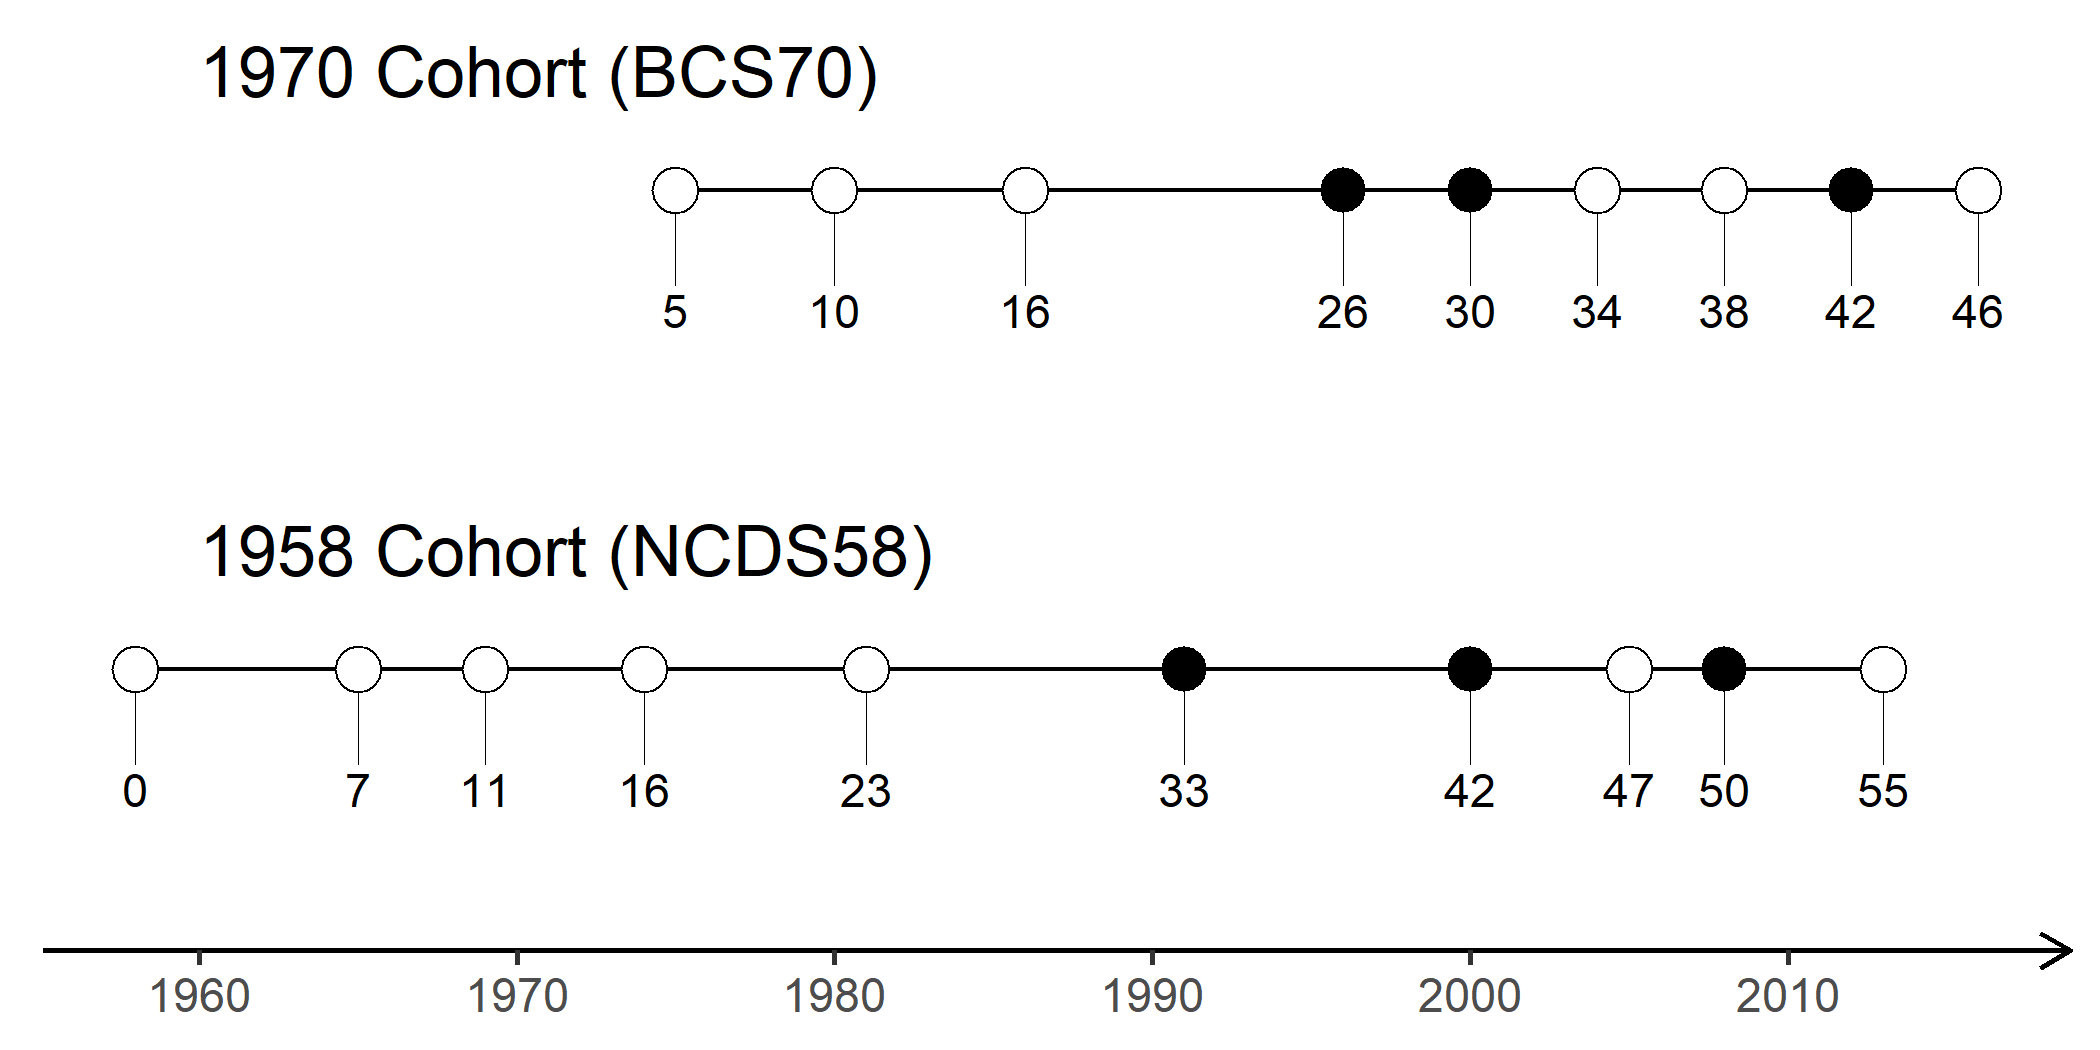
\includegraphics[width=\linewidth]{chap3/graphic/data-itw-values.png}
    \hrulefill
	\vspace{-3em}
	\justify\singlespacing\footnotesize{\textit{Notes:} This figure presents the timing of interviews for the NCDS58 and BCS70 cohorts. Circles correspond to interviews and numbers under them indicate the age of cohort members during this interview. Full circles correspond to interviews for which attitudes can be derived. The horizontal arrow at the bottom of the figure represents the years.}
\end{figure}
% Attitudes available
The full circles on the figure indicate interviews from which values can be derived, thus I will focus on those years for the remaining of the paper.
% Periods definition
I define four periods according to the decade in which individuals belong, i.e. their twenties, thirties, forties, or fifties.
% BCS periods
For the BCS70 cohort, I refer to period 1 for the interview at the age of 26, to period 2 for the one at 30, and to period 3 for the one at 42.
% NCDS periods
For the NCDS58 cohort, periods start at period 2 for the interview at the age of 33, then period 3 corresponds to the one at 42, and period 4 refers to the one at 50.

% Attrition ?
One of the main issues with cohort studies is attrition. 
% Either missing interviews OR lose them
Cohort members do not participate at every interview and therefore some individuals are either missing at some interviews or lost definitely at some point.
%
Table \ref{chap3-tab:data-resp} presents the responses rates by periods of interest.
% Table to show attrition
\begin{table}[!tb]
    \centering
    \caption{Number of individuals and response rates by periods.}
    \label{chap3-tab:data-resp}
    \begin{threeparttable}
        \setlength{\tabcolsep}{15pt}
        
\begin{tabular}{lrr}
\toprule
  & \multicolumn{1}{c}{BCS} & \multicolumn{1}{c}{NCDS}\\
\midrule
Initial & 19,006 (100\%) & 17,885 (100\%)\\
\midrule
Period 1 & 9,003 (47.4\%) & \\
Period 2 & 11,261 (59.2\%) & 11,469 (64.1\%)\\
Period 3 & 9,841 (51.8\%) & 11,419 (63.8\%)\\
Period 4 &  & 9,790 (54.7\%)\\
\midrule
All & 6,115 (32.2\%) & 8,107 (45.3\%)\\
\bottomrule
\end{tabular}

        \begin{tablenotes}[flushleft]
            \footnotesize{\item \textit{Notes}: Response rates between parentheses. The last row corresponds to individuals who have been interviewed at all periods.}
        \end{tablenotes}
    \end{threeparttable}
\end{table}
%
The second-period interview is the one with the greater response rate, i.e. 64.1\% for the NCDS58 cohort and 59.2\% for the BCS70 one. This latter interview, when BCS70 cohort members are 30, has been conducted at the same time as the third-period interview for the NCDS58 cohort, when they are 42, so in the year 2000. Thus, they share the same set of variables.

\subsection{Motivational types of values}

% Attitudes from statements
I derive values from individuals' answers to statements about their attitudes.\footnote{In social psychology, an attitude toward an object---such as a statement---corresponds to emotions, beliefs, and behaviors toward this particular object.} At each interview, cohort members answer to statements using a 5-level scale (strongly disagree / disagree / neither agree nor disagree / agree / strongly agree). I attribute them a score for each statement between -2 and 2 according to the answer.

% Group statement by categories
These statements cover several attitudes and can be grouped into categories (in alphabetical order): Anti-Racism (AR), Authority (A), Children (C), Environment (E), Inequality Aversion (IA), Information Technology (IT), Learning (L), Morale (MOR), Political Cynicism (PC), Work-Ethic (WE), and Working Mother (WM). 
The full list of statements are reported in appendix \ref{chap3-statement}. Some examples of statements are the following:
\begin{table}[!h]
    % \footnotesize
    \renewcommand*{\arraystretch}{1.5}
	\begin{tabular}{rl}
    (A2)    & \textit{For some crimes the death penalty is the most appropriate sentence};\\
    (MOR3)  & \textit{Couples who have children should not separate};\\
    (PC1)   & \textit{None of the political parties would do anything to benefit me};\\
    (WE1)   & \textit{Having almost any job is better than being unemployed}.
    \end{tabular}
\end{table}

% Compute the average score
\noindent I compute the average score within each attitude category for each individual at each period. Thus, each individual has a score for each attitude in each period. Then, I standardize each attitude score at the cohort and period level. Thus, each individual belongs to a cohort and has, for each period, a standardized score for each attitude that is relative to her cohort in a given period.

%
Nonetheless, the number of available statements depends on the cohort and the period. Table \ref{chap3-tab:data-available-short} summarizes the number of available statements at each interview.
\begin{table}[!tb]
    \centering
    \caption{Number of available statements at each interview}
    \label{chap3-tab:data-available-short}
    \begin{threeparttable}
        \setlength{\tabcolsep}{12pt}
        \begin{tabular}{lrrrrrr}
\toprule
\multicolumn{1}{c}{} & \multicolumn{3}{c}{BCS70} & \multicolumn{3}{c}{NCDS58} \\
\cmidrule(l{3pt}r{3pt}){2-4} \cmidrule(l{3pt}r{3pt}){5-7}
Attitude & 26 & 30 & 42 & 33 & 42 & 50\\
\midrule
Authority & 4 & 6 & 3 & 6 & 6 & 3\\
Anti-Racism &  & 5 & 2 & 5 & 5 & 3\\
Children &  & 4 & 2 & 2 & 4 & \\
Environment &  & 3 & 2 & 3 & 3 & 3\\
Inequality Aversion & 1 & 7 & 5 & 7 & 7 & 3\\
Info. Techno. &  & 4 &  &  & 4 & \\
Learning &  & 4 &  &  & 4 & \\
Morale & 3 & 6 & 3 & 6 & 6 & 3\\
Political Cynicism & 3 & 3 & 3 & 3 & 3 & 3\\
Work Ethic & 2 & 3 & 3 & 3 & 3 & 3\\
Working Mother &  & 5 & 2 &  & 5 & \\
\bottomrule
\end{tabular}
        \begin{tablenotes}[flushleft]
            \footnotesize{\item \textit{Notes}: This table presents the number of available statements in each attitudes at each age for the NCDS58 and BCS70 cohorts. Details on statements are reported in the appendix, see tables \ref{chap3-tab:statement-split-1}, \ref{chap3-tab:statement-split-2} and \ref{chap3-tab:statement-split-3} in appendix \ref{chap3-statement}.}
        \end{tablenotes}
        \end{threeparttable}
\end{table}
%
Thus, interviews do not necessarily share the same set of statements, except when the BCS70 cohort is 30 and the NCDS58 cohort is 42 because interviews were performed using the same questionnaires.

I derive motivational types of values from these attitude scores. I focus on the five attitudes that are available in all interviews in order to have the same baseline for each period of both cohorts. These attitudes are Authority (A), Inequality Aversion (IA), Morale (MOR), Political Cynicism (PC), and Work Ethic (WE).

%
I use a Principal Component Analysis (PCA) to transform the 5-dimension attitudes into the two-dimension motivational types of values. PCA increases the interpretability of vectors while minimizing the information loss. By focusing on the two first components, which are orthogonal by the construction of the PCA, I can interpret them as the two main values that discriminate and, therefore, characterize individuals in their attitudes. 

The other principal components act as residuals to some extent. Although they might be incorporated into the analysis, Proposition \ref{chap3-prp:relevant} states that a value needs to be sufficiently discriminatory between groups in order to be relevant in the group membership decision. The two first principal components capture more than 50\% of the explained variance in attitudes, which makes the discriminatory power of the other principal components less relevant.
% \footnote{PCA allows to determine values by summarizing attitudes through dimension reduction which reduces the noise in attitudes, hence, this noise is relegated to the unused components that explain the smaller part of the variance and are not relevant.} Therefore, I focus on the two first components.

%
I perform PCA at the cohort and period level. Figure \ref{chap3-fig:data-pca-v5} presents the eigenvectors of the two first principal components.
\begin{figure}[!tb]
    \centering
    \caption{Eigenvectors of the two first principal components}
    \label{chap3-fig:data-pca-v5}
    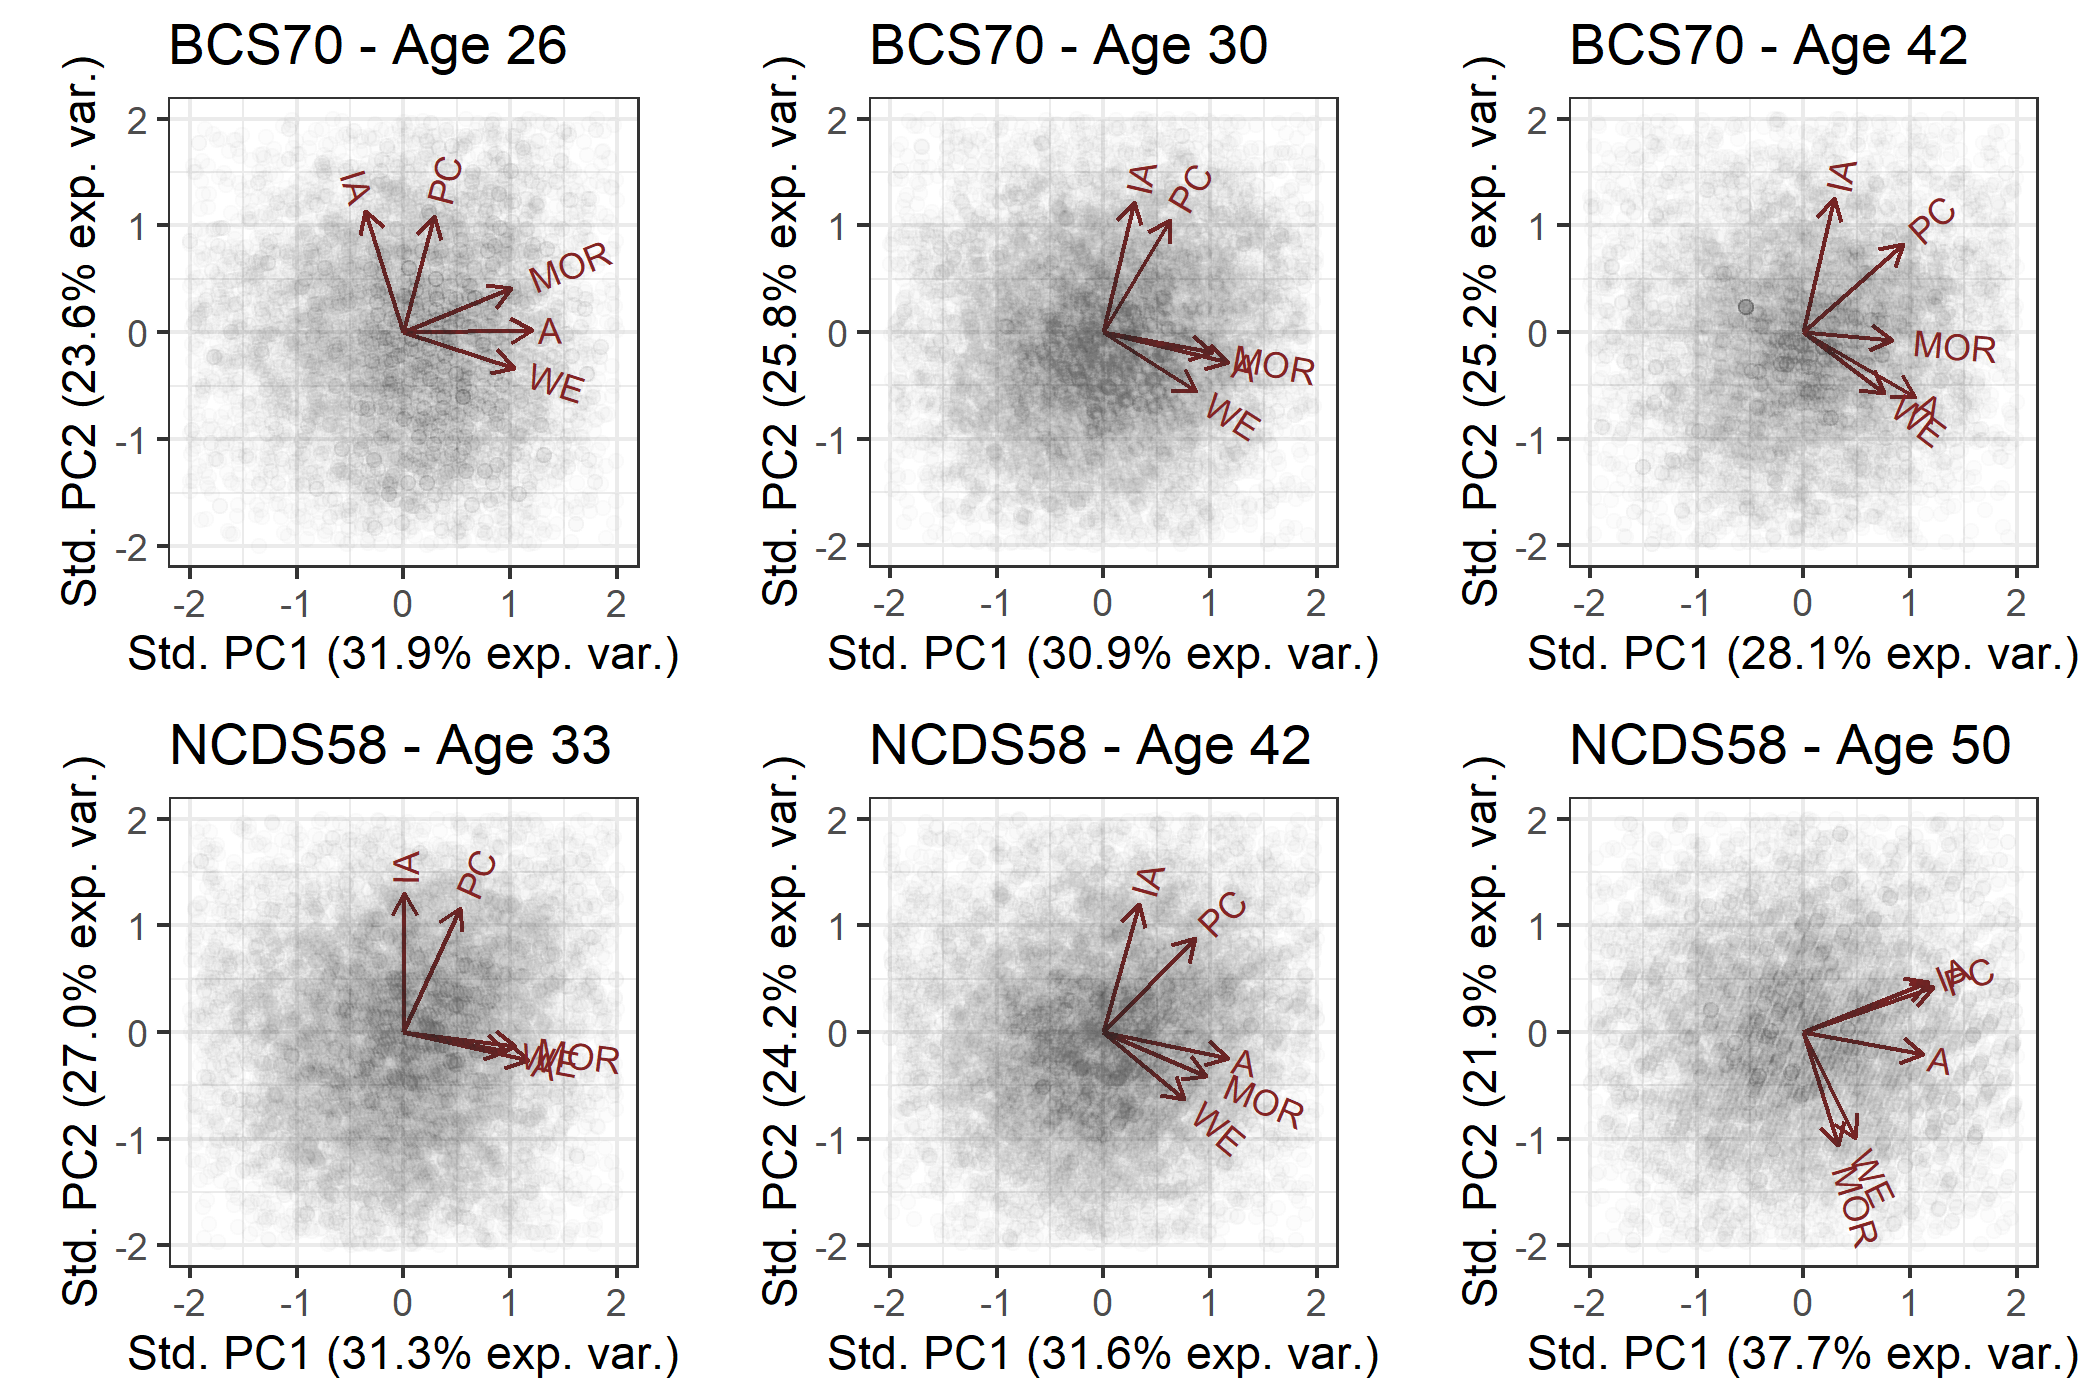
\includegraphics[width=\linewidth]{chap3/graphic/pca-v5.png}
    \hrulefill
	\vspace{-3em}
	\justify\singlespacing\footnotesize{\textit{Notes:} This figure presents the eigenvectors of the two first principal components. Details on the eigenvectors are available in tables \ref{chap3-tab:pca-v5-BCS70} and \ref{chap3-tab:pca-v5-NCDS58}, respectively for the BCS70 and NCDS58 cohorts. Attitudes are Authority (A), Inequality Aversion (IA), Morale (MOR), Political Cynicism (PC) and Work Ethic (WE).}
\end{figure}
Links between attitudes are fairly stable across cohorts and periods. These principal components explain more than 50\% of the variance in attitudes. I interpret both of them as the two-dimensional structure of universal motivational types of values, as introduced by \citet{Schwartz1992Universals, Schwartz2012Overview}---see figure \ref{chap3-fig:schwartz} in the appendix.

% PC1
Focusing on the first principal component (PC1), the x-axis directions of vectors highlight attitudes that characterize \textit{conservatism} which is the preference for stability, security, tradition, and conformity. In the data, they reflect a taste for attitudes about Authority, Morale, and Work Ethic. Thus, the dimension that discriminates the most between individuals is \textit{conservatism} (versus \textit{progressivism}).
% PC2
The second principal component (PC2) is orthogonal to the previous dimension of values at the cohort-period level. Focusing on the y-axis directions of vectors, they indicate attitudes that characterize \textit{collectivism}. This motivational type of values refers to the care and concern about others, reflecting universalism and benevolence. In the data, this value is associated with attitudes toward Political Cynicism and aversion for Inequality and Work Ethic. Therefore, the second discriminatory dimension between individuals is \textit{collectivism} (versus \textit{individualism}).\footnote{In the terms of \citet{Schwartz1992Universals}, both dimensions are respectively named conservation (versus openness-to-change) and self-transcendence (versus self-enhancement).}

% Projection
I make a projection of both principal components for all individuals at each period.  Thus, each cohort member has a Conservatism score ($Cons$) and a Collectivism score ($Coll$) at each period. By construction, both scores are standardized at the cohort-period level and \textit{orthogonal}. Thus, the values are not inter-dependent \textit{per se}. The inter-dependency arises with socio-economic characteristics---such as gender, education, etc.---once they are introduced as control variables. These covariates capture several dimensions of groups to which individuals identify, hence, it creates inter-dependency between values as they are correlated among groups.

\subsection{Groups mapping using political vote}

In my theoretical framework, the agent belongs to a group and the spillover effect occurs once the agent identifies with another group. Defining groups is therefore crucial to understand spillover effects as we expect individuals to change groups along with their values. So far, a group can be interpreted as composed of peers with whom the agent identifies in terms of values. One can think about those peers as close people such as relatives, neighbors, or colleagues; since we tend to share values with them. Nonetheless, most of the time, individuals cannot freely break off all ties with those latter as there may be direct costs. These direct costs thwart the identification of changes in group membership as they introduce noise through bonds. Thus, I cannot rely on peers to define groups.

An alternative proxy for groups is political vote. There is no direct cost in voting for one party or another at the general election, conditional on voting. In addition, political parties reflect part of individuals' values in the sense that the agent decides to identify with one party with respect to others when voting.

Figure \ref{chap3-fig:vote-v5} presents a mapping of values of the average voters for each main political party at the closest general election (GE); see table \ref{chap3-tab:data-vote} in appendix \ref{chap3-details} for the shares of vote in both cohorts.
\begin{figure}[!tb]
    \centering
    \caption{Average values according to political vote}
    \label{chap3-fig:vote-v5}
    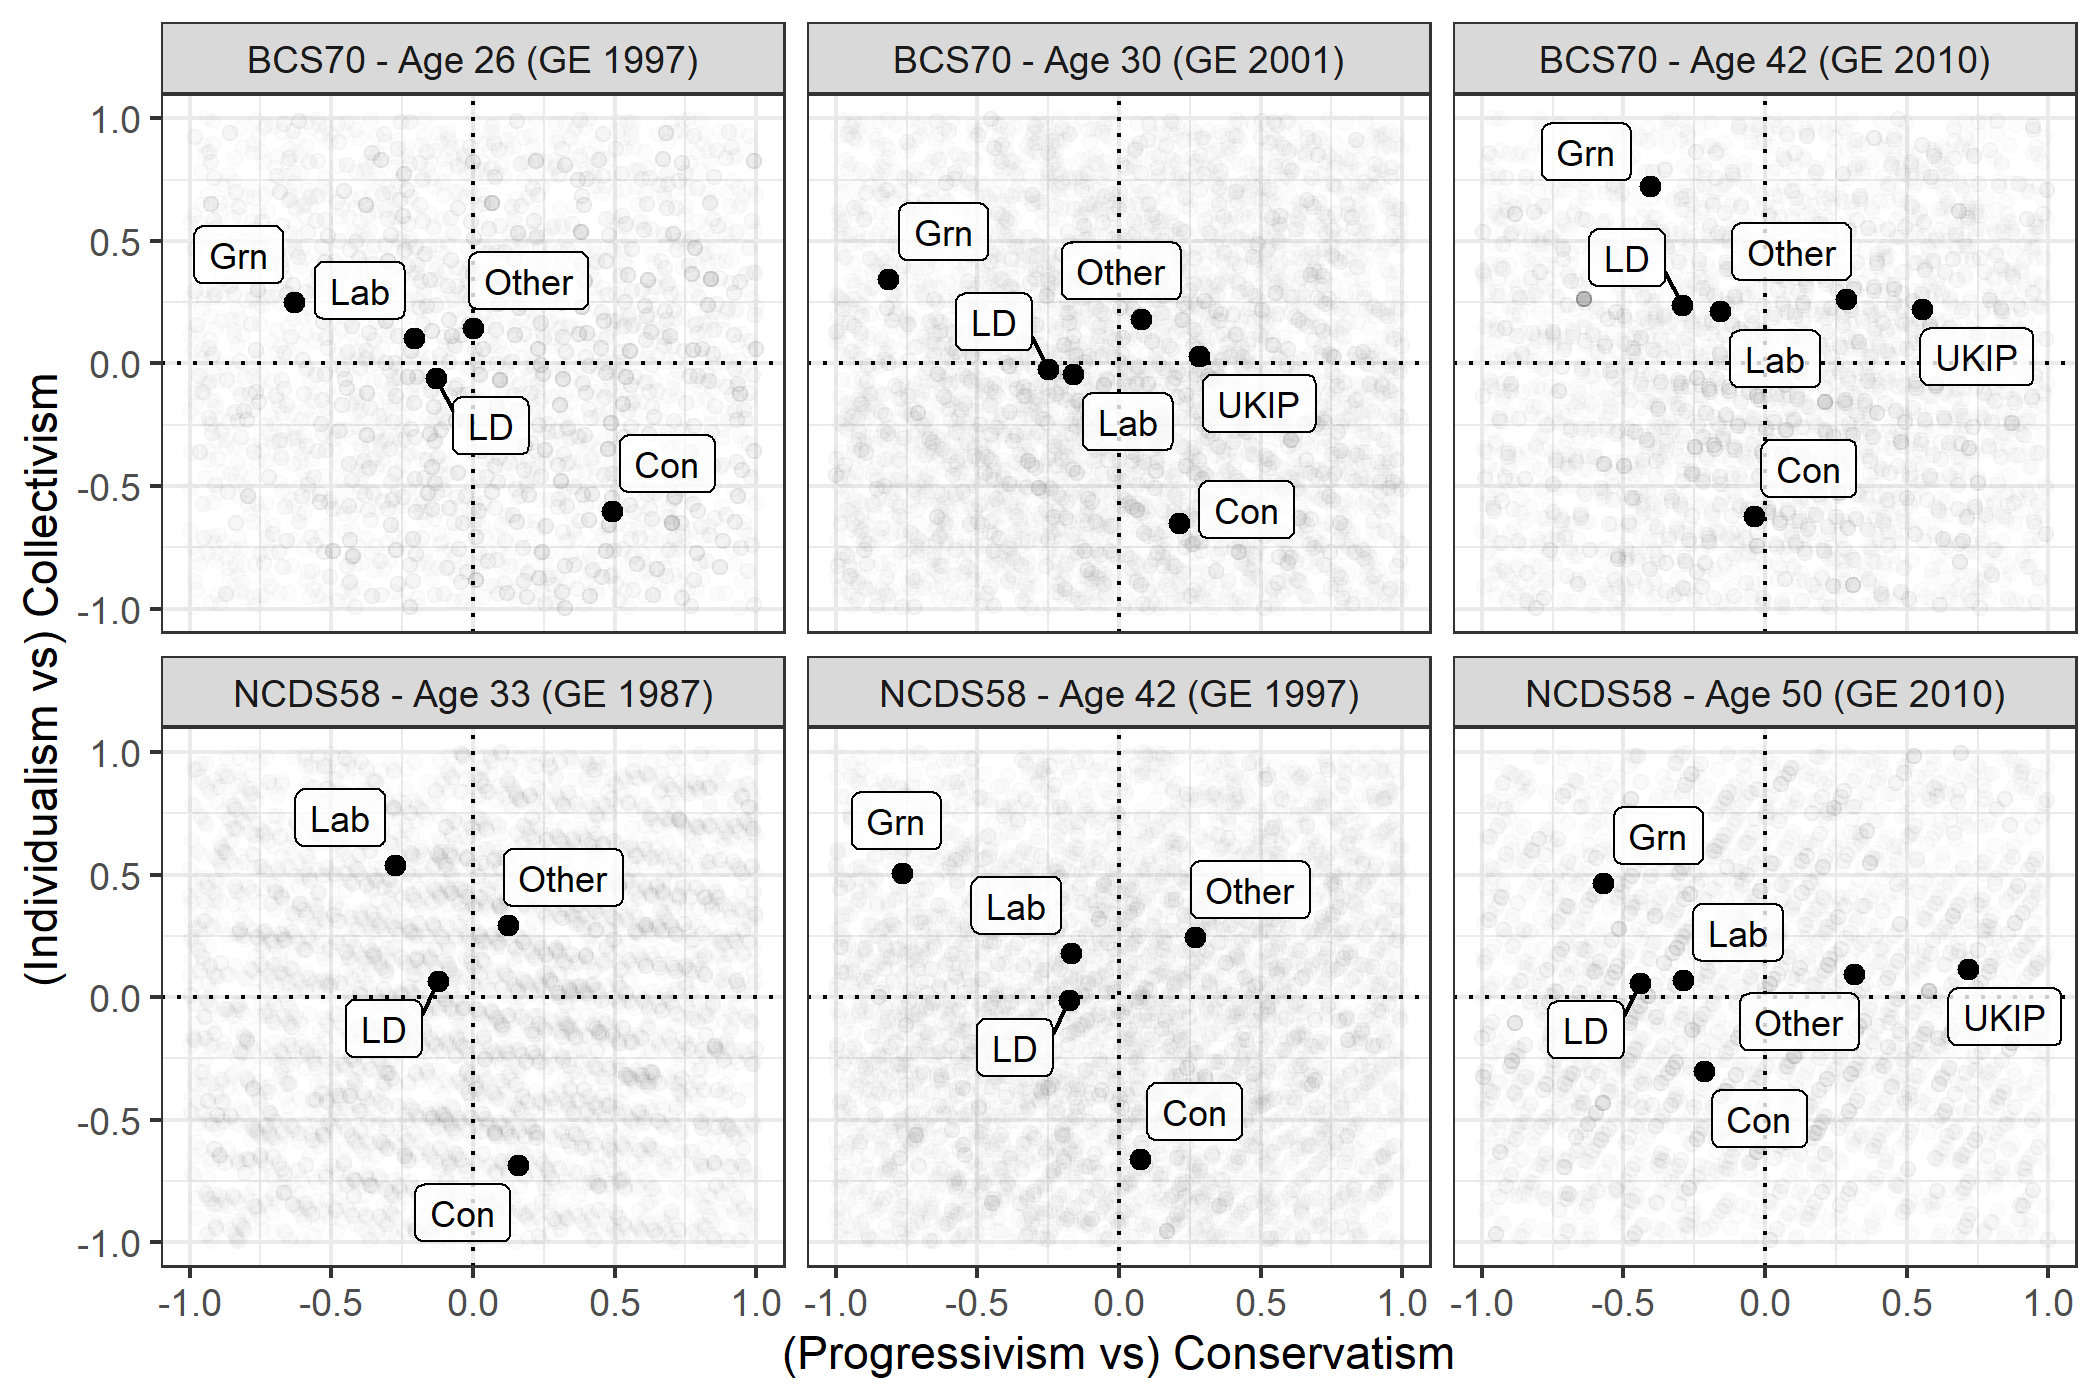
\includegraphics[width=\linewidth]{chap3/graphic/vote-v5.png}
    \hrulefill
	\vspace{-3em}
	\justify\singlespacing\footnotesize{\textit{Notes:} This figure presents the mapping of average scores in conservatism and collectivism according to political voting in General Elections (GE). Political parties are (in alphabetical order): Conservative (Con), Green (Grn), Labour (Lab), Liberal Democrat (LD), and UK Independence Party (UKIP). Other encompasses all other parties, blank votes and abstention.}
\end{figure}
% 1987 GE
The bottom-left panel represents the mapping of values in the 1987 General Election for which only the NCDS58 cohort voted at age 33. Positioning of the two main UK political parties is consistent: Labour (Lab) voters are progressive and collectivist, whereas Conservative (Con) voters are conservative and individualist. The Liberal Democrats (LD) provides an in-between the Labour and Conservative parties.\footnote{Note that the Liberal Democrats party only appeared in 1988 as the merge of the SDP–Liberal Alliance that was running into general elections in 1987. For the ease of exposition, I refer to the SDP–Liberal Alliance in 1987 as the Liberal Democrats.}
Other encompasses all other parties, blank votes, and abstention.
% 1997 GE
The top-left and bottom-mid panels correspond to the 1997 General Election. The Green party (Grn) emerged and attracted voters with progressive and collective values. The overall structure of values and voting is stable across cohorts.
% 2001 GE
The top-mid panel shows the rise of the far-right party UKIP for the 2001 General Election. As the formation of political parties is endogenous, it is unsurprising that it emerged in an area where there was no political supply.
% 2010 GE
Both right panels depict the political mapping for the 2010 general election. The average political voters of the BCS70 cohort are more spread along the collectivism axis, while those in the older cohort are rather spread on the conservatism axis.

Positionings of political parties relative to each other are consistent---over time and across cohorts---on the two-dimensional values' space. Thus, I consider the political vote of individuals as a proxy of their group membership in the remaining of the empirical analysis. This proxy helps understand how individuals start to identify with other groups after life-changing events.

\subsection{Life-changing events}

We are interested in life events that generate information shocks on conservatism ($Cons$) or collectivism ($Coll$) in order to show whether there exist spillover effects or not. The type of life events that I have to consider to test this hypothesis requires two properties: \textit{exogeneity} and \textit{non-reversibility}.
On the one hand, the life event has to be exogenous so that values in the previous period do not influence the likelihood that the life event occurs. 
On the other hand, the life event has to be non-reversible. Otherwise, the probability to reverse the event is likely to be endogenous which would bias the estimate of individual's values at the time of interviews.\footnote{Note that life events that provide temporary shocks are also interesting to study. Especially if a temporary shock leads to a change in groups. In the absence of reverse shock, both---time and group---consistencies would prevent the individual to come back to her previous group's values. Thus, a sufficiently large temporary shock can have long-run consequences on individuals' values.}

In this regard, I focus on two life events that satisfy both properties, namely, \textit{to have ever had cancer} and \textit{to have a girl as first child conditional on having a baby}.
%
The former life event is exogenous in the sense that values, such as conservation and collectivism, do not affect the probability to have cancer---excluding individuals with lung cancer. It is also non-reversible as I compare individuals who have \textit{ever} had cancer with respect to those who never had one. I set the focus on the information shock related to the fact that people have known they have cancer, not on the illness \textit{per se} as someone might have one without knowing it.
Note that for the older cohort at age 50, there may be a bias when considering the effect of this life event on values. As people turn 50, they expect that their health condition will deteriorate in the coming years, thus, they may anticipate such a life event and change their values beforehand. This potential mechanism would bias my estimate toward zero as the control group---those who did not get cancer yet---anticipate and shift their values in the same direction as those who have been treated. Therefore, for this cohort at that age, my approach is likely to provide a lower bound estimate of the effect of having ever had cancer on values.

For the latter life event, I consider a sub-sample that only contains individuals who have at least one baby, hence, I compare those who had a girl as a first child with those who got a boy.
Thus, the life event is exogenous to values because the probabilities of child's sex at birth are fifty-fifty, considering that sex‐selective abortion is very rare in the UK.\footnote{
\citet{Dubuc2007Increase} argue that sex-selective abortion occurs among mothers born in India and living in Britain. They show that sex ratios at birth have always been one point lower for Asian groups in England and Wales before 1990. Although this issue raises several social and economic concerns, it does not statistically affect my results as they represent a minority in the data.} Once the baby is born, the life event is non-reversible because it has occurred and remains forever.
I do not also consider adopted children because the sex may be decided by parents and therefore linked to values and preferences (\citealt{Dahl2008Demand}). I also exclude stillborn babies because the socialization of parents with the baby does not occur.\footnote{Note that this tragic life event could also be considered as a potential life event that would deeply affect values.}

%
I only focus on the first child as fertility decisions for following children might be linked to the sex of the eldest child and values, e.g. a preference for diversity in children's birth sex. Moreover, some parents may have a boy as their first child and a girl thereafter. Some changes in values may be specific to having a girl even though she is not the first baby. Thus, this is likely to produce a lower-bound estimate and also to reduce the statistical power of effects of this life event on values.

Lastly, I study the role of unemployment on values as it is a sizeable information shock in individuals' life. Nonetheless, I cannot use it as a life event to show the existence of spillover effects among values because it does not satisfy both properties. First, individuals change their activity status quite often and, therefore, the effect of unemployment on values is all the time affected by these changes in status. Second, the likelihood to be unemployed is clearly endogenous to values. For instance, one might argue that individuals with high work ethic, hence high conservatism and high individualism, have a lower probability to be unemployed as they are less likely to quit their job with respect to people with low work ethic.

\subsection{Variables and summary statistics}

%%%%% LIFE EVENT VARIABLES %%%%%
For life events, I focus on three of them: to have had a girl as a first child, to have ever had cancer, and to have ever been unemployed. $GirlFirst$ is a dummy variable that equals one if the sex of the first child is female, and zero if it is a male. $GotCancer$ is also a dummy variable that equals one if the individual has ever had cancer by the time of the interview. $BeenUnemp$ is a dummy variable that equals one if the individual has ever been unemployed at least one month by the time of the interview. 
% Activity history
Activity status is derived from the full activity histories to the nearest month since cohort members are 16 years old. These data are available for all cohort members until the last interview they have participated in. When individuals were missing in previous interviews, interviewers asked them about their activities during the period until then.

%%%%% SOCIO-ECONOMIC CHARACTERISTICS %%%%%
I consider several socio-economic characteristics as control variables that will introduce the inter-dependency between values. Among them, I use the sex at birth of cohort members and their level of education based on the highest academic qualification they obtained. $Female$ is a dummy variable that equals one if the cohort member is born as a female. I regroup education levels into three categories that characterize primary, secondary, and tertiary education levels ($Educ$). 

%%%%% SUMMARY STATISTICS %%%%%
Table \ref{chap3-tab:data-statdesc} presents the descriptive statistics for the NCDS58 and BCS70 cohorts. Both cohorts contain respectively 30,552 and 27,906 observations. Period variables corresponds to dummy variables to determine the decade in which individuals are.
\begin{table}[!tb]
    \centering
    \caption{Summary statistics}
    \label{chap3-tab:data-statdesc}
    \begin{threeparttable}
        \setlength{\tabcolsep}{5pt}
        
\begin{tabular}{lrrrrrrrrrr}
\toprule
\multicolumn{1}{c}{} & \multicolumn{5}{c}{NCDS58 - N = 30,552} & \multicolumn{5}{c}{BCS70 - N = 27,906} \\
\cmidrule(l{3pt}r{3pt}){2-6} \cmidrule(l{3pt}r{3pt}){7-11}
Variable & Mean & SD & Min & Max & NA & Mean & SD & Min & Max & NA\\
\midrule
Period 1 - Twenties &  &  &  &  &  & 0.31 & 0.46 & 0 & 1 & 0\\
Period 2 - Thirties & 0.35 & 0.48 & 0 & 1 & 0 & 0.40 & 0.49 & 0 & 1 & 0\\
Period 3 - Forties & 0.37 & 0.48 & 0 & 1 & 0 & 0.29 & 0.45 & 0 & 1 & 0\\
Period 4 - Fifties & 0.28 & 0.45 & 0 & 1 & 0 &  &  &  &  & \\
Female & 0.51 & 0.50 & 0 & 1 & 0 & 0.53 & 0.50 & 0 & 1 & 0\\
Education - Primary & 0.62 & 0.49 & 0 & 1 & 0 & 0.52 & 0.50 & 0 & 1 & 0\\
Education - Secondary & 0.19 & 0.39 & 0 & 1 & 0 & 0.19 & 0.39 & 0 & 1 & 0\\
Education - Tertiary & 0.20 & 0.40 & 0 & 1 & 0 & 0.29 & 0.46 & 0 & 1 & 0\\
Girl First & 0.49 & 0.50 & 0 & 1 & 7199 & 0.48 & 0.50 & 0 & 1 & 14789\\
Got Cancer & 0.03 & 0.16 & 0 & 1 & 0 & 0.01 & 0.12 & 0 & 1 & 0\\
Been Unemployed & 0.34 & 0.48 & 0 & 1 & 0 & 0.21 & 0.41 & 0 & 1 & 0\\
\bottomrule
\end{tabular}

        \begin{tablenotes}[flushleft]
            \footnotesize{\item \textit{Notes}: This table presents the descriptive statistics of variables used in the study. Values and attitudes are not displayed in this table as they are standardized.}
        \end{tablenotes}
    \end{threeparttable}
\end{table}
